\chapter{Introduction}

{\red Intro paragraph here.}

\section{Motivation}
\label{section:Motivation}

\subsection{Threat Model}
From the perspective of verification, we would like to have confidence
that the file system is secure purely based on the file system's security
specification.  This means that we have to treat the developer of the
file system with an adversarial mindset. More specifically, we assume the developer may be malicious and intentionally deliver an implementation that can be exploited in the future, which we call \emph{an adversarial implementation}.
This subsumes all possible bugs that a well-meaning but error-prone developer might introduce into the implementation as well as any implementation that is designed to be exploited.

As a result, our threat model is that the adversary both develops the
file system and runs an adversarial application on top of the file system
in an attempt to obtain confidential file data.  However, the adversary
does provide a proof that their file-system implementation meets our
security specification.  The potential victim runs on top of the same
file system but sets their permissions so that the confidential files
are not accessible to the adversary's process.  Our goal is to ensure
that the security specification is so strong that it prevents leaks even
when the file-system developer is colluding with adversarial processes
running on top of the file system.

Our threat model is focused on proving that the file-system implementation has
no confidentiality bugs, rather than proving the absence of bugs in the
environment outside of the file system. Thus, we assume that our model
of how the file-system implementation executes is correct.  That is, we are not
concerned with bugs in unverified software or hardware outside of the file
system, or users mounting malicious disk images.  We do prove that
\texttt{mkfs} produces a correct image, but ensuring confidentiality on top of an
intentionally corrupted file system image is difficult, even without formal
verification. We also do not reason about timing channels, as we do not model time.

\subsection{Challenges}
\label{s:goal:chal}

A difficult aspect of formally proving the security of a file system lies
in guaranteeing confidentiality.  This is difficult because of four challenges:

\paragraph{1. Two-safety.}
First, proving confidentiality is more difficult than
proving functional correctness: because, confidentiality
is a two-safety property.  Functional correctness is a one-safety
property because a violation of functional correctness can be demonstrated
by a single execution.  For instance, if an application wrote one byte to
a file and then read back a different byte, this single execution shows
that the file system is incorrect.  Thus, functional correctness
of a file system is a theorem that says that all executions meet the
spec (i.e., there are no such violations).  Integrity properties,
such as ensuring that one user cannot corrupt another user's data,
are an example of a one-safety functional-correctness property and can
be handled using standard verification techniques.

In contrast, demonstrating a violation of confidentiality requires
two executions, where the results observed by an adversary differ depending on
the secret data.
%% %% TODO: We don't do this though. Maybe find a better example for this?
For instance, consider a file system with block-level deduplication that
also exposes the number of free blocks.  An adversary who wants to
learn the contents of a victim's file could write their guess for the
victim's block into the adversary's own file and then check whether
the number of free blocks stayed the same or decreased.  If the file
system implemented deduplication across users, this attack allows an
adversary to learn whether their guess block was already present in the
file system, thus inferring whether the victim has that data.

In the above example, looking at a single execution does not allow one
to directly conclude that data was leaked, because the system appears
to be functioning correctly.  Determining that data is leaking requires
one to consider a pair of executions, in which the adversary performs
the same operations, but the confidential user data is different.
If these two executions produce different adversary-observable results,
the adversary is able to infer information about confidential data.

By stating confidentiality as a two-safety property, the above
deduplication example would violate confidentiality, and thus could not
appear in an implementation that was proven to achieve confidentiality.
Specifically, suppose the starting states of the two executions differed
in the contents of a confidential file, where in one execution the file
matched the adversary's guess and in the other execution it didn't match.
In this case, the number of free blocks returned by the adversary
would differ in the two executions, which would not be allowed by the
confidentiality definition.

\paragraph{2. Nondeterministic specifications.}
Another challenge in proving confidentiality lies in the fact
that many specifications, including those in the file system, are
nondeterministic.  Some nondeterminism is unavoidable because file
systems must deal with crashes (e.g., due to power failure), which can
occur at any time.  Thus, it is impossible to
know what are the exact contents of the disk after a crash; the on-disk
state could reflect any prefix of the writes issued by the file system.
Modern disks complicate this situation even further by buffering writes
in memory inside the disk controller; as a result, the writes can be
made durable out-of-order, and the state of the disk after a crash might
reflect some out-of-order writes.  Even in the absence of crashes, the
file system implementation may want to use randomness (e.g., to randomize
directory hash tables), which makes the execution non-deterministic.

Other nondeterminism comes from specifications that hide irrelevant
details.  For instance, the inode allocator in the file system does
not specify which precise inode number will be returned; instead,
its specification simply states that it will return
\emph{some} inode number that is not already in use.

Any nondeterminism is a potential leak of confidential data.  The
nondeterministic specification of the block allocator from above does not
preclude the allocator from leaking confidential data, because it could,
in theory, choose the next inode number based on the confidential contents
of files, without violating its specification (i.e., still returning some
unused inode number).

Even the nondeterminism associated with the state of the disk
after a crash can be taken advantage of by an adversarial file-system
implementation to leak data.  For instance, a high-performance
file-system specification allows the file system to delay flushing data
to disk.  An adversarial implementation could choose whether to flush
data immediately or defer the flush based on one bit of confidential
data from a victim's file.  To take advantage of this, an adversary
could wait for the system to crash and, after the crash, check whether
any writes appear to have been lost.  If so, the adversary concludes
the file system must have deferred the writes, which would have only
happened if the confidential bit was zero.  This, in turn, can allow
the adversary to infer confidential bits.

\paragraph{3. Non-uniform outcome probabilities.}
Another challenge arises because an adversary may obtain
more precise information about the system by executing the same program repeatedly.
Such an action will allow the adversary to approximate \emph{frequencies} of
different outcomes of a program. which some confidential information may be inferred from. A simple example of this challenge can be seen in figure \ref{fig:Frequency_Leaking_Program}.

\begin{figure}[H]
\centering
    \begin{verbatim}
    if (get_random_bit() == 1)
      return secret_bit
    else
      return get_random_bit()
    \end{verbatim}
\caption{Example of a program that leaks information via return value frequencies}
\label{fig:Frequency_Leaking_Program}
\end{figure}

This code leaks the secret bit 50\% of the time and outputs a random bit 50\% of the time. It is also important to note that it can output 0 or 1 independently of the secret value. This way, any (state, return) pair represents a successful execution. Therefore, by observing just a single return value, an adversary cannot infer the value of the secret bit. However, the frequencies of the output values in table \ref{table:Return_value_distribution} shows that they correlate with the value of the secret bit.

\begin{figure}[H]
    \centering
\begin{tabular}{| c | c | c |}
	\hline
	Secret bit & Output \% 0 & Output \% 1 \\
	\hline
	0 &	75\% & 25\% \\
	\hline
	1 &	25\% & 75\% \\
	\hline
\end{tabular}
\caption{Distributions of return values for each state.}
\label{table:Return_value_distribution}
\end{figure}

Any adversary who can observe the output of this program sufficiently many times can infer the value of the secret bit with high confidence. These types of vulnerabilities are not limited to usage of randomization. They also manifest themselves when there are random events such as crashes that can affect the behavior of the system.

\paragraph{4. Indirect disclosure.}
Yet another challenge is that an adversarial
file system might not immediately leak confidential data.  For example,
an adversarial file system may wait for a legitimate user to read
confidential data, at which point the file system would be allowed to
access this data, since it has to return it to the user.  However, in
addition to returning this data, an adversarial file system could also
stash away a copy of it, so that the adversary can later retrieve it.
For instance, the file system could change the order of entries in an
on-disk directory structure, or change the allocated inode numbers or
block numbers, based on the confidential data that it wants to leak.
Preventing this attack is difficult because the adversarial file system
appears to have legitimate access to the user's data when operating on
behalf of that user.

\paragraph{5. File-system complexity.}
Finally, file systems are complex software. Linux ext4, for
instance, consists of approximately 50,000 lines of code.  Even the simple
verified DFSCQ file system consists of thousands of lines of executable
code~\cite{chen:dfscq}.  The proofs of functional correctness for DFSCQ
are already tens of thousands of lines of Coq code. The complexity of
proving two-safety, which is a more challenging property, could easily
spiral out of control.

\section{State of the Art: Information Flow Control}
De facto approach to specifying confidentiality is through the information flow control. An information flow control policy restricts and regulates transfer of information between different parts of the system.

One widely used confidentiality specification in information flow control literature is called \emph{noninterference}. Informally, noninterference states that "unprivileged users (a.k.a. low users) should observe the same behavior from the system regardless of a privileged users' (a.k.a. high users) actions in the system". Noninterference is formalized in many different computation models. In this thesis, we use the state-machine model since it fits better to the systems we create.

Although its widespread usage, noninterference is not suitable for many storage systems. The reason for that is it prohibits any transfer of information, both direct and indirect. However, storage systems sometimes expose effects of privileged users indirectly via metadata or some public information of the system like available free space. For example, in a file system, if a privileged user creates a file and writes to it, other users of the file system may see that he created a file, even though they may not see the file's contents. For many applications, this behavior is completely acceptable, even though noninterference prohibits it. Because of this, storage systems require a more flexible confidentiality specification.

\section{Solution Approaches}
We took two different approaches to address the mentioned challenges: (1) sealed blocks and data noninterference, and (2) nondeterminism oracles, abstractions and refinements. These approaches complement each other, and together, offer a solution to each of the challenges. 

Our first approach sealed blocks and data noninterference addresses challenges 1, 2, 4, and partially 5. Sealed blocks reduce the two-execution property to a trace property, which is a one-execution property. Data noninterference allows nondeterministic specifications while preventing exploitation of such nondeterminism by implementation. Both of them reduced required proof effort significantly but required us to make simplifications in our implementation.

Second approach solves the challenges that first approach falls short.Nondeterminism oracles enable reasoning of individual nondeterministic events. This ability leads to a stricter confidentiality specification that prevents challenge 3, while still being flexible enough to prevent overly-verbose specifications. Abstractions and refinements encapsulate the complexity in small components and allow complex systems to be implemented in a modular fashion while keeping proof complexity in check. 

We briefly explain all of the approaches below. We present more detailed explanations in the following chapters.

\subsection{Sealed Blocks and Data Noninterference}
Sealed blocks and data noninterference are our first attempt at addressing the challenges. Our implementation of these approaches address many of the challenges but also reveal the intricacies of specifying and proving confidentiality of storage systems, most notably challenge 3. Sealed blocks and data noninterference is briefly explained below.

\paragraph{Sealed Blocks}
We used sealed blocks approach to address challenge 1, that confidentiality proofs being harder and more complex than integrity proofs by turning two-execution proofs into trace properties, which require one-execution proofs. Key idea behind sealed blocks is that if a program's behavior does not depend on confidential data, then it is not possible for it to leak confidential data; since it will behave the same no matter what the data is. Sealed blocks achieve this via two mechanisms: (1) providing a way to handle data without accessing its contents, and (2) enforcing access control when the contents are accessed. 

First mechanism achieved via an operation we call \emph{sealing}. It takes a piece of data and "seals" it with the owner of the data, by turning it into an abstract object that does not provide any functionality other than \emph{unsealing} it. This way, showing that a program's behavior does not depend on confidential data reduces into showing that it only handles the sealed data. Which can be done by a static analysis of the program.

However there is still fair amount of functionality that requires inspecting the contents of the data, especially for systems that uses on-disk data structures. An example of this is the bitmap of an allocator. To be able to allocate or free any resources,  it has to inspect and modify the contents of a bitmap. Second mechanism allows that while ensuring the program does not access any data that it is not permitted to access. Since sealed data require unsealing to access to the contents, each unseal operation can be detected and recorded during the execution, creating an \emph{unseal trace}. With unseal traces, showing that a program does not leak confidential data reduces to showing that its unseal trace only contains unseals that it is permitted to do so. This turns a two-execution proof into a one-execution proof because a program's unseal trace can be obtained by examining a single execution.

\paragraph{\red Data Noninterference}
We defined data noninterference as a solution to traditional noninterference being too strong for storage systems confidentiality. Data noninterference embodies the insight "if a program's behavior doesn't depend on confidential data, then it cannot leak confidential data via its return value". 

\iffalse
{\red Not sure where to put this following part. Probably will be here so I am keeping it here for now.}\\
{\red .....}\\
At the core of the two-execution style noninterference definition lies the notion of "equivalent states" and preservation of that equivalence throughout the execution of the system. An informal description of noninterference can be stated as "a program is noninterfering when the program is executed from equivalent states, it preserves the equivalence of the resulting states and returns the same values". This description ensures two things: (1) states cannot be distinguished from a program's return values, (2) after-execution states cannot be distinguished in the future by running other noninterfering programs. A formalism of two-execution style noninterference can be seen in figure \ref{fig:NI_Definition}.

\begin{figure}[H]
    \centering
    \begin{verbatim}
    Definition Noninterference
        {T} (p: prog T) 
       (R: state -> state -> Prop):=
      forall (s1 s2: state) (r1: T),
        exec s1 p (s1', r1) ->
        R s1 s2 ->
        exists s2' r2,
            exec s2 p (s2', r2) /\
            R s1' s2' /\
            r1 = r2.
    \end{verbatim}
    \caption{Formalization of two-executions noninterference}
    \label{fig:NI_Definition}
\end{figure}
{\red .....}\\

{\red .....}\\
A good way define equivalence of the states is "two states are equivalent if they are the same for their non secret parts". This definition makes all states equivalent to each other in our example, because the state is a single secret bit. Since any pair of state and return value is a valid execution, it is possible to find another execution from a related state with same return value. Therefore, this implementation satisfies the noninterference definition. 

Figure \ref{fig:NI_Matching_Paths} illustrates how each execution matches with another from an equivalent state. Each arrow represents a possible execution of the program. On the labels, numbers in the brackets represent generated random bits, and the number following the brackets denotes the return value. Executions are colored based on their return values.
We can see that, for each execution, there is an execution with the same color  from the equivalent state.

\begin{figure}[H]
    \centering
    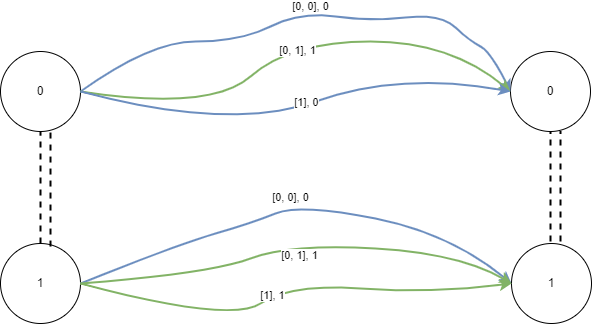
\includegraphics[scale=0.5]{templates/figures/matching-paths.png}
    \caption{Visualisation of \ref{fig:Frequency_Leaking_Program} satisfying noninterference.}
    \label{fig:NI_Matching_Paths}
\end{figure}

Although our example satisfies noninterference, the secret bit can be determined via the observed frequency of repeated calls.
{\red .....}\\
\fi

\subsection{Nondeterminism Oracles, Abstractions and Refinements}
Our second group of approaches addresses the challenges that is left unresolved by the first group. Nondeterminism oracles, abstractions and refinements incorporate the insights we obtained from our first attempt to obtain stronger specifications.

\paragraph{Nondeterminism Oracles}
Our approach to addressing challenge 3 is developing a technique to reason about each possible nondeterministic event individually. Such a technique enables confidentiality specifications that can require return value equality to hold for each possible nondeterministic event. If the return value equality holds for each nondeterministic event, then there are equal number of executions from equivalent states that leads to a particular return value, which implies that observed frequencies of return values will be preserved.

We achieved this via a technique we call \emph{nondeterminism oracles}. A nondeterminism oracle is an abstract object that, whenever the execution needs to make a nondeterministic choice, it "asks" oracle and chooses based on the oracle's answer. Therefore different oracles lead to different executions of the same program. Similarly, for a fixed oracle, execution becomes deterministic. This allows us to enforce return value frequencies to be the same by requiring return value equality for each oracle.

\paragraph{Abstractions and Refinement}
To tackle the complexity of file systems, we use abstractions. Being able to define abstractions at a desired points help containing and compartmentalizing the complexity in the system and reduces the proof complexity as implementations stack on top of each other. In our work, we use refinement for connecting abstractions to implementations where correction of the refinement is established by simulation proofs.

One possible complication is that it is known that noninterference is not necessarily preserved under simulations \ref{}. However nondeterminism oracles lead to a confidentiality specification that is preserved under simulations given that refinement satisfies a certain property. This condition will be explained in more detail in the following chapters.


\subsection{Implementations}
We implement our solution approaches in two frameworks: sealed blocks and data noninterference are implemented in DiskSec, and nondeterminism oracles, abstractions and refinements are implemented in ConFrm. To test the frameworks, We implement two file systems: SFSCQ for DiskSec, and ConFs for ConFrm. All the frameworks and systems are implemented in Coq proof assistant. They are extracted to Haskell to produce runnable code. Details of these frameworks and file systems will be explained in their respective chapters.

\section{Contributions}
There are four categories of contributions of this thesis: (1) proof strategies, (2) confidentiality specifications, (3) implementations of frameworks for confidentiality reasoning, and (4) confidential file systems with machine-checkable proofs.

\subsubsection*{Proof Strategies}
\begin{itemize}
\item Sealed blocks, a proof approach that factors out reasoning about confidentiality
  from most of the storage system code.
  
\item Oracles, a proof approach for reasoning about specific series of nondeterministic events.

\item Reboot functions, a proof approach for reasoning about specific outcome of a nondeterministic reboot process.

\item A meta-theory for preservation of RDNI through abstractions, including a modified simulation definition that incorporates oracles, reboot functions, and crash-reboot-recovery process.
\end{itemize}

\subsubsection*{Confidentiality Specifications}
\begin{itemize}
\item Data Noninterference, a confidentiality specification based on noninterference that captures discretionary access control and deals with nondeterminism due to crashes.

\item RDNI, a confidentiality specification based on noninterference that incorporates oracles, and reboot functions, and crash-reboot-recovery process. RDNI provides stronger guarantees than data noninterference under nondeterminism.
\end{itemize}

\subsubsection*{Framework Implementations}
\begin{itemize}
\item DiskSec, a framework for specifying and proving confidentiality 
for storage systems that reduces proof effort by using sealed block approach.

\item ConFrm a framework for specifying and proving confidentiality that implements RDNI and its meta-theory. ConFrm provides support for implementing systems as layers of abstractions, defining refinements, and proving simulations.

\end{itemize}

\subsubsection*{Confidential File Systems}
\begin{itemize}
\item SFSCQ, the first file system with a machine-checked proof of
  confidentiality. SFSCQ uses data noninterference as its specification, 
  and DiskSec for proving its confidentiality

\item ConFs, a first file system that uses checksum-based, encrypted logging with a machine-checked confidentiality proof. ConFs is implemented in ConFrm and uses RDNI as its confidentiality specification.

\item An evaluation that compares SFSCQ and ConFs to demonstrate the performance overheads of each approach.
\end{itemize}

\subsection{Limitations}
Both of our systems have certain limitations such as:

\begin{itemize}
    \item Both systems have termination insensitive specifications.
    \item DiskSec does not allow comparison of confidential data.
    \item SFSCQ has to execute recovery as the super user.
    \item ConFrm does not provide a program logic to help with proving properties of programs.
    \item ConFrm does not provide any help for proving confidentiality of the highest abstraction layer.
    \item ConFs does not have a buffer cache for fast reads and writes, 
          indirect block pointers in inodes, or file names and directory structures.
    \item Both SFSCQ and ConFs has simple access control mechanisms.
\end{itemize}     

\section{Outline}
Chapter \ref{chapter:Related_work} presents the related work in the literature. Chapter \ref{chapter:Disksec} explains proof ideas behind Disksec and its implementation details. Chapter \ref{chapter:SFSCQ} presents SFSCQ, first formally verified file system with a confidentiality specification. Chapter \ref{chapter:ConFrm} describes ConFrm, a confidentiality framework for implementing systems modularly and with strong guarantees regarding nondeterminism. Chapter \ref{chapter:ConFs} presents the structure and implementation of ConFs. Chapter \ref{chapter:Evaluation} evaluates the performance of both file systems. Chapter \ref{chapter:Conclusion} concludes the thesis.



\iffalse
%%%%Explain the reason why there are two and how they compare to each other.

%%%% Whole story here security expensive etc...
{\red From Proposal}
As computation and storage shift toward the cloud, the safety of computation and data is becoming increasingly important. Users expect their data stored in such systems to stay secret against malicious third parties. Precise descriptions of how such a system should behave to ensure confidentiality of the stored data are called confidentiality specifications. A confidentiality specification of a system both forces a system to maintain certain properties, and informs users about the safety guarantees that system provides. 

Writing a confidentiality specification is generally more difficult than writing a correctness specification. To demonstrate the possible hardships of writing a specification that can prevent malicious implementations, we can look at a specification for the create() operation from our confidential file system ConFs. create() takes an owner and creates an empty file owned by the provided owner. Upon successful completion, it returns the inode number that identifies the file. A natural correctness specification for its return value could be “create() returns the index of the previously unused inode that now corresponds to the newly created file.” If we were only interested in functional correctness, this would be an acceptable specification. However, there is a substantial confidentiality problem associated with it. create() is allowed to return any inode number as long as it was unused at the time of the call. A malicious implementation of the file system can take advantage of this nondeterminism in the specification to pick the returned inode number and subsequently leak confidential data, e.g., last byte of the return value being equal to the first byte of a block that belongs to another user.

This problem, and others of the same nature, could be solved by writing a fully deterministic specification for create() that exactly pinpoints what it should return and what the file-system state should be after its completion. However, such a specification runs the risk to be overly verbose to a degree that specification is the implementation, obscuring the important parts of the specification, making it difficult to read and comprehend, and defeating one of the key purposes of writing a specification. Therefore, a good confidentiality specification should address such vulnerabilities in its scope, but should also abstract implementation details so it can be read, understood, and reviewed by humans. Finding the right balance between these conflicting requirements is what makes writing a confidentiality specification challenging.

Our proposed solution to the above problems is ConFrm, a framework for 
implementing and proving the confidentiality of storage systems in a modular fashion. ConFrm provides a noninterference definition with better guarantees for nondeterministic behavior, as well as the required tools and necessary conditions for safety-preserving abstractions. These two components of ConFrm enable us to overcome the limitations of previous works and provide a simple yet powerful tool for implementing safe storage systems out of composable components..


To test the capabilities of ConFrm, we implemented ConFS, a confidential file system that is crash-resistant via checksum logging, transactional operations, and coarse-grained discretionary access control. 

Both ConFrm and ConFS are implemented in Coq. All proofs are fully machine-checked to ensure their correctness. 

{\color{red}From Disksec}
Many security problems today stem from bugs in software.  Although there
has been significant effort in reducing bugs through better testing,
fuzzing, model checking, and so on, subtle bugs remain and continue
to be exploited.  Machine-checked verification is a powerful approach
that can eliminate a large class of bugs by proving that an
implementation meets a precise specification.

Prominent examples of machine-checked security proofs include verification of
strict isolation (with confidentiality) for an OS kernel in CertiKOS~\cite{costanzo:certikos-infoflow},
seL4~\cite{murray:sel4-infoflow}, and Komodo~\cite{ferraiuolo:komodo}, as well as security proofs in Ironclad~\cite{hawblitzel:ironclad} about applications
like a password hasher and a notary service.  However, proving the
security of systems with rich sharing semantics, such as file systems,
is an open problem.  For example, unlike prior examples that focus on
strict isolation without controlled sharing, users in a file system
can share files with one another, and the underlying implementation
has shared data structures (such as a buffer cache or write-ahead log)
that contain data from different users.

Proving security for a file system requires addressing two key challenges.
The first challenge lies in \emph{specifying} security. Integrity can be
expressed as simply as a functional correctness property. Confidentiality is more
challenging to specify. For example, consider
a natural specification for \cc{readdir}, which allows the file system to return
the names in a directory in any order.  This nondeterminism could be
abused by a buggy or malicious file system to leak confidential file
data through careful manipulation of the order of \cc{readdir} results.
Furthermore, nondeterminism is essential to a file system, because file
systems must deal with crashes, which can occur nondeterministically
at any time.

One approach to specifying confidentiality is to formulate it as a
noninterference property, such as in most information-flow-control
systems.  This means that the execution of one process (a potential victim
processing confidential data) cannot influence the execution of another
process (an adversary trying to learn that data).  Noninterference can
be stated concisely, and is easy for applications to use.  However,
information-flow-control style guarantees are stronger than what file
systems aim for.  Instead, file systems aim for weaker notions of
confidentiality, along the lines of discretionary access control on
files that reveal some metadata, such as file lengths.

A second challenge lies in proving confidentiality.  Confidentiality is a
``two-safety'' property~\cite{terauchi:safety}, which requires reasoning
about \emph{pairs} of executions to show that an adversary cannot observe
any differences correlated with confidential data.  However, reasoning
about pairs of executions is more complicated than reasoning about a
single execution, which is sufficient for proving integrity and functional correctness.

% note: recent paper on this, Cartesian Hoare Logic for Verifying k-Safety
% Properties from PLDI 2016. There are other attempts at this that are simpler
% and targetted towards security.

This paper presents \sys, an approach for proving the security, and
specifically confidentiality, for storage systems, such as file systems.
The paper demonstrates the benefits of \sys by developing, specifying,
and proving the security of a file system in a prototype called \sfscq,
based on the DFSCQ file system~\cite{chen:dfscq}.

\sys addresses the specification challenge by using a notion of \emph{data
noninterference} that both matches what file systems aim to provide
and is concise and easy to use for applications.  Data noninterference
requires that an adversary's execution be independent of the contents of
individual files, but it allows the adversary to observe other metadata,
such as file length and directory entries, and allows for discretionary
access control (i.e., a user can choose to disclose their data).

To address the challenge of proving security, \sys factors out reasoning
about confidentiality from all other properties, such as functional
correctness.  \sys does so by introducing a notion of sealed blocks.
This builds on the intuition that file systems do not look inside of the
blocks that represent user file contents.  As a result, \sys is able to
treat confidential file blocks as opaque in much of the file-system code,
greatly reducing the need for manual proofs of two-safety that consider
pairs of executions.  The only manual proofs of two-safety are in the
top-level \cc{read} and \cc{write} system calls.

We implemented \sys and \sfscq in the Coq proof assistant~\cite{coq}.  All proofs of security are
machine-checked by Coq, eliminating the possibility of bugs that
violate \sfscq's specification.  An evaluation of \sfscq shows that its
specifications are complete enough to prove confidentiality of a simple
application.  The evaluation also shows that \sys's approach allowed us
to develop \sfscq with a modest amount of effort, and that \sfscq achieves
comparable performance to the DFSCQ file system that it is based on.

The contributions of this paper are:

\begin{CompactItemize}

\item \sfscq, the first file system with a machine-checked proof of
  confidentiality.  \sfscq has a concise specification that captures
  discretionary access control using data noninterference, and deals
  with nondeterminism due to crashes.

\item \sys, an approach for specifying and proving confidentiality
  for storage systems that reduces proof effort.  \sys uses the
  idea of sealed blocks to factor out reasoning about confidentiality
  from most of the file system code.

\item An evaluation that demonstrates that \sys's approach leads to
  negligible performance overheads in \sfscq, that it precludes the
  possibility of confidentiality bugs that have been found in existing
  file systems, and that \sfscq's specification allows applications to
  reason about their confidentiality.

\end{CompactItemize}

Our \sfscq prototype has several limitations.
Since it relies on Coq's extraction to Haskell, inherited from DFSCQ,
its trusted computing base (TCB) includes the Haskell runtime and
compiler.
The version of \sfscq with fully machine-checked proofs does not support
changing permissions.
A newer version of \sfscq supports dynamic permissions but has a
few proofs that have not been repaired to reflect this change.
Finally, \sfscq's access-control mechanisms are relatively simple,
supporting owned and public files but not groups or separate read and
write permissions.

\fi
